\setAuthor{Jaan Kalda}
\setRound{lõppvoor}
\setYear{2005}
\setNumber{G 10}
\setDifficulty{10}
\setTopic{Staatika}

\prob{Platvorm}
\begin{wrapfigure}[9]{r}{0.3\textwidth}
	\begin{center}
		\vspace{-20pt}
		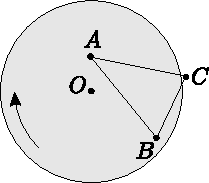
\includegraphics[width=\linewidth]{2005-v3g-10-yl}
	\end{center}
\end{wrapfigure}
Siledas põrandas on pöörlev ringikujuline platvorm (joonisel pealtvaates, hall), mis on samast materjalist nagu põrandki (joonisel valge). Põranda ja platvormi ülemine pind on samal horisontaaltasandil. Kolm ühesugust keha ühendatakse kergete varraste abil kolmnurgaks ning asetatakse sedasi, et kaks keha asuvad platvormil punktides $A$ ja $B$ (vt joonist). Vardad ei puuduta ei põrandat, ega platvormi.\\
\osa Kui kolmas keha lebaks põrandal punktis $C$, kas siis kolmnurk hakkaks põranda suhtes liikuma või jääks paigale? Põhjendage vastust.\\
\osa Märkige joonisel selline punktihulk $X$, kus võiks asuda kolmas keha nii, et kolmnurk jääks põranda suhtes paigale.

\emph{Märkus:} kolmnurga külgede $AC$ ja $BC$ pikkusi võib muuta. Seega, kui kolmas keha asub punktis $D \in X$, siis üldjuhul $|AD| \neq |AC|$ ja $|BD| \neq |BC|$.

\hint
Tasakaalu korral peab kehtima jõumomentide tasakaal. Kuna kehade süsteemile mõjuvad kolm jõudu, peavad jõudude pikendused lõikuma samas punktis, sest vastasel juhul saaksime valida kahe jõu pikenduse lõikepunkti ning selle punkti suhtes mõjuks kolmanda punkti poolt nullist erinev jõumoment. Lisaks paneme tähele, et kehadele $A$ ja $B$ mõjuvad sama absoluutväärtusega jõud (mõlemad on libisemise äärel) ning nende suunad on teada.

\solu
\osa Kolmnurk hakkab põranda suhtes liikuma, sest summaarne jõumoment punkti $C$ suhtes koosneb kahest liidetavast, mis omavad ühte ja sama märki ning on nullist erinevad. Selles veendumiseks tuleb tõmmata punktidesse $A$ ja $B$ rakendatud hõõrdejõudude pikendused $AE$ ja $BE$ ($E$ on nende pikenduste lõikepunkt), mis on risti vastavalt raadiustega $OA$ ja $OB$ (vt joonist).\\
\osa Süsteemile mõjub kolm horisontaalsuunalist jõudu. Jõumomentide tasakaalu tingimusest järeldub et nende jõudude pikendused peavad lõikuma ühes punktis $E$. Olgu kolmas keha punktis $D$. Siis punkti $D$ rakendatud hõõrdejõud peab olema suunatud piki sirget $ED$. Teisest küljest, jõudude tasakaalu tingimusest lähtuvalt peavad hõõrdejõudude vektorid moodustama võrdhaarse kolmnurga $\vec F_A+\vec F_B+\vec F_C = 0$ (võrdhaarse, sest punktidesse $A$ ja $B$ rakendatud jõud on moodulilt võrdsed, |$\vec F_A| = |\vec F_B|$).

\begin{center}
	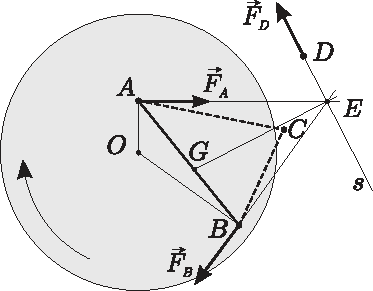
\includegraphics[width=0.7\linewidth]{2005-v3g-10-lah}
\end{center}

Selletõttu peab vektorite $\vec F_A$ ja $\vec F_D$ vaheline nurk võrduma vektorite $\vec F_D$ ja $\vec F_B$ vahelise nurgaga. Niisiis peab sirge $ED$ ristuma nurga $\angle AEB$ poolitajaga $EG$. See tähendab, et punktihulgaks $X$ on sirge $s$, mis ristub nurga $\angle AEB$ poolitajaga $EG$. Lõpetuseks paneme tähele, et hõõrdejõud $\vec F_D$ peab olema moodulilt väiksem, kui $\vec F_A$ ja $\vec F_B$, sest muidu toimuks kolmanda keha juures libisemine. Nii ka on, sest nurk $\angle AEB$ on väiksem kui \ang{60} (\ang{60}, st võrdkülgse kolmnurga puhul oleks jõudude kolmurgas $\vec F_A + \vec F_B + \vec F_C = 0$ kõik küljed võrdsed, \ang{60} väiksemate nurkade puhul aga oleks vektor $\vec F_C$ oma moodulilt teistest väiksem).
\probend